\begin{frame}
  \frametitle{GDB: GNU Project Debugger}
  \fontsize{11}{11}\selectfont
  \begin{columns}[T]
    \column{0.8\textwidth}
    \begin{itemize}
    \item The debugger on GNU/Linux, available for most embedded
      architectures.
    \item Supported languages: C, C++, Pascal, Objective-C, Fortran,
      Ada...
    \item Command-line interface
    \item Integration in many graphical IDEs
    \item Can be used to
      \begin{itemize}
      \item control the execution of a running program, set
        breakpoints or change internal variables
      \item to see what a program was doing when it crashed: post
        mortem analysis
      \end{itemize}
    \item \url{https://www.gnu.org/software/gdb/}
    \item \url{https://en.wikipedia.org/wiki/Gdb}
    \item New alternative: {\em lldb} (\url{https://lldb.llvm.org/})\\
      from the LLVM project.
    \end{itemize}
    \column{0.2\textwidth}
    
\includegraphics[width=0.9\textwidth]{common/gdb.png}
  \end{columns}
\end{frame}

\begin{frame}[fragile]
  \frametitle{GDB crash course (1/3)}
  \begin{itemize}
    \item GDB is used mainly to debug a process by starting it with {\em gdb}
    \begin{itemize}
      \item \code{$ gdb <program>}
    \end{itemize}
    \item GDB can also be attached to running processes using the program PID
    \begin{itemize}
      \item \code{$ gdb -p <pid>}
    \end{itemize}
    \item When using GDB to start a program, the program needs to be run with
    \begin{itemize}
      \item \code{(gdb) run [prog_arg1 [prog_arg2] ...]}
    \end{itemize}
  \end{itemize}
\end{frame}

\begin{frame}
  \frametitle{GDB crash course (2/3)}
  \small
  A few useful GDB commands
  \begin{itemize}
  \item \code{break foobar} (\code{b})\\
    Put a breakpoint at the entry of function \code{foobar()}
  \item \code{break foobar.c:42}\\
    Put a breakpoint in \code{foobar.c}, line 42
  \item \code{print var}, \code{print $reg} or \code{print task->files[0].fd} (\code{p})\\
    Print the variable \code{var}, the register \code{$reg} or a more
    complicated reference. GDB can also nicely display structures with all
    their members
  \item \code{info registers}\\
    Display architecture registers
  \end{itemize}
\end{frame}

\begin{frame}
  \frametitle{GDB crash course (3/3)}
  \small
  \begin{itemize}
  \item \code{continue} (\code{c})\\
    Continue the execution after a breakpoint
  \item \code{next} (\code{n})\\
    Continue to the next line, stepping over function calls
  \item \code{step} (\code{s})\\
    Continue to the next line, entering into subfunctions
  \item \code{stepi} (\code{si})\\
    Continue to the next instruction
  \item \code{finish}\\
    Execute up to function return
  \item \code{backtrace} (\code{bt})\\
    Display the program stack
  \end{itemize}
\end{frame}

\ifthenelse{\equal{\training}{debugging}}
{
\begin{frame}
  \frametitle{GDB advanced commands (1/3)}
  \small
  \begin{itemize}
    \item \code{info threads} (\code{i threads})\\
      Display the list of threads that are available
    \item \code{info breakpoints} (\code{i b})\\
      Display the list of breakpoints/watchpoints
    \item \code{delete <n>} (\code{d <n>})\\
      Delete breakpoint <n>
    \item \code{thread <n>} (\code{t <n>})\\
      Select thread number <n>
    \item \code{frame <n>} (\code{f <n>})\\
      Select a specific frame from the backtrace, the number being the one
      displayed when using \code{backtrace} at the beginning of each line
  \end{itemize}
\end{frame}

\begin{frame}
  \frametitle{GDB advanced commands (2/3)}
  \small
  \begin{itemize}
    \item \code{watch <variable>} or \code{watch \*<address>}\\
      Add a watchpoint on a specific variable/address.
    \item \code{print variable = value} (\code{p variable = value})\\
      Modify the content of the specified variable with a new value
    \item \code{break if condition == value}\\
      Break only if the specified condition is true
    \item \code{watch if condition == value}\\
      Trigger the watchpoint only if the specified condition is true
    \item \code{x/<n><u> <address>}\\
      Display memory at the provided address. \code{n} is the amount of memory to
      display, \code{u} is the type of data to be displayed (\code{b/h/w/g}).
      Instructions can be displayed using the \code{i} type.
  \end{itemize}
\end{frame}

\begin{frame}
  \frametitle{GDB advanced commands (3/3)}
  \small
  \begin{itemize}
    \item \code{list <expr>}\\
      Display the source code associated to the current program counter location.
    \item \code{disassemble <location,start_offset,end_offset>} (\code{disas})\\
      Display the assembly code that is currently executed.
    \item \code{p function(arguments)}\\
      Execute a function using GDB. NOTE: be careful of any side effects that
      may happen when executing the function
    \item \code{p $newvar = value}\\
      Declare a new gdb variable that can be used locally or in command sequence
    \item \code{define <command_name>}\\
      Define a new command sequence. GDB will prompt for the sequence of
      commands.
  \end{itemize}
\end{frame}
}
{
\subsection{Remote debugging}
}

\begin{frame}
  \frametitle{Remote debugging}
  \begin{itemize}
  \item In a non-embedded environment, debugging takes place using \code{gdb}
    or one of its front-ends.
  \item \code{gdb} has direct access to the binary and libraries compiled
    with debugging symbols.
  \item However, in an embedded context, the target platform
    environment is often too limited to allow direct debugging with
    \code{gdb} (2.4 MB on x86).
  \item Remote debugging is preferred
    \begin{itemize}
    \item \code{ARCH-linux-gdb} is used on the development workstation, offering
      all its features.
    \item \code{gdbserver} is used on the target system (only 400 KB
      on arm).
    \end{itemize}
  \end{itemize}
  \begin{center}
    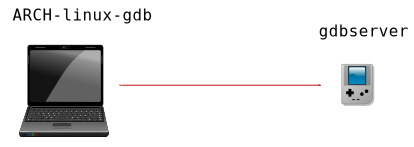
\includegraphics[width=0.5\textwidth]{common/gdb-vs-gdbserver.pdf}
  \end{center}
\end{frame}

\begin{frame}
  \frametitle{Remote debugging: architecture}
  \begin{center}
    \includegraphics[width=\textwidth]{common/gdb-vs-gdbserver-architecture.pdf}
  \end{center}
\end{frame}

\begin{frame}
  \frametitle{Remote debugging: usage}
  \begin{itemize}
  \item On the target, run a program through \code{gdbserver}.\\
    Program execution will not start immediately.\\
    \code{gdbserver :<port> <executable> <args>}
    \code{gdbserver /dev/ttyS0 <executable> <args>}
  \item Otherwise, attach \code{gdbserver} to an already running program:\\
    \code{gdbserver --attach :<port> <pid>}
  \item Then, on the host, start \code{ARCH-linux-gdb <executable>},\\
    and use the following \code{gdb} commands:
    \begin{itemize}
    \item To tell \code{gdb} where shared libraries are:\\
      \code{gdb> set sysroot <library-path>} (typically path to build space without \code{lib/})
    \item To connect to the target:\\
      \code{gdb> target remote <ip-addr>:<port>} (networking)\\
      \code{gdb> target remote /dev/ttyUSB0} (serial link)
    \end{itemize}
  \end{itemize}
\end{frame}

\begin{frame}
  \frametitle{Coredumps for post mortem analysis}
  \begin{itemize}
  \item When an application crashes due to a {\em segmentation fault}
    and the application was not under control of a debugger, we get no
    information about the crash
  \item Fortunately, Linux can generate a \code{core} file that
    contains the image of the application memory at the moment of the
    crash, and gdb can use this \code{core} file to let us analyze the
    state of the crashed application
  \item On the target
    \begin{itemize}
    \item Use \code{ulimit -c unlimited} in the shell starting the
      application, to enable the generation of a \code{core} file
      when a crash occurs
    \item The output name for the coredump file can be modified using
      \code{/proc/sys/kernel/core_pattern}.
    \item See \manpage{core}{5}
    \end{itemize}
  \item On the host
    \begin{itemize}
    \item After the crash, transfer the \code{core} file from the target to
      the host, and run
      \code{ARCH-linux-gdb -c core-file application-binary}
    \end{itemize}
  \end{itemize}
\end{frame}
